% ---------------------------------------------------------------------------
% Figure 1 -- Two-tier Oversight Game pipeline (standalone TikZ source)
%   pdflatex fig_architecture.tex   ->   fig_architecture.pdf
%   Colors: colF (Frontier F), colW (Workers W), colH (Human Overseer H)
% ---------------------------------------------------------------------------
\documentclass[11pt,border=0.6pt]{standalone}
% ---------------------------------------------------------------------------
% Shared preamble for the proposal's schematic figures:
%   fig_architecture.tex   (Figure 1, pipeline)
%   fig_policies.tex       (Figure 2, the four deferral policies)
%   fig_specialization.tex (Figure 6, expected harm and team loss heatmaps)
% Uses the unified three-role semantic palette:
%   colW (Cobalt Blue)        -- Workers (W)
%   colF (Royal Crimson-Plum) -- Frontier Orchestrator (F)
%   colH (Forest Emerald-Teal)-- Human Overseer (H)
% ---------------------------------------------------------------------------
\usepackage[T1]{fontenc}
\usepackage{lmodern}
\DeclareFontFamily{OML}{lmm}{\skewchar\font127 }
\DeclareFontShape{OML}{lmm}{m}{it}{<-> lmmi10}{}
\DeclareFontShape{OML}{lmm}{b}{it}{<-> lmmib10}{}
\DeclareFontFamily{OMS}{lmsy}{\skewchar\font48 }
\DeclareFontShape{OMS}{lmsy}{m}{n}{<-> lmsy10}{}
\DeclareFontShape{OMS}{lmsy}{b}{n}{<-> lmbsy10}{}
\DeclareFontFamily{OT1}{lmr}{\hyphenchar\font45 }
\DeclareFontShape{OT1}{lmr}{m}{n}{<-> rm-lmr10}{}
\DeclareFontShape{OT1}{lmr}{bx}{n}{<-> rm-lmbx10}{}
\DeclareFontShape{OT1}{lmr}{m}{it}{<-> rm-lmri10}{}
\usepackage[scaled=0.90]{helvet}
\usepackage{amsmath,amssymb}
\usepackage{tikz}
\usetikzlibrary{arrows.meta,calc}

% ---- three-role semantic palette + neutral/outcome accents ------------------
\definecolor{colW}{RGB}{25,100,186}     % Workers (W): Cobalt Blue
\definecolor{colF}{RGB}{157,23,77}      % Frontier Orchestrator (F): Royal Crimson-Plum
\definecolor{colH}{RGB}{15,118,94}      % Human Overseer (H): Forest Emerald-Teal
\definecolor{primary}{RGB}{157,23,77}   % alias for Frontier tier (F)
\definecolor{worker}{RGB}{25,100,186}   % alias for Worker tier (W)
\definecolor{human}{RGB}{15,118,94}     % alias for Human Overseer (H)
\definecolor{accent}{RGB}{22,138,69}    % safe / harm-detected shield
\definecolor{gatec}{RGB}{71,85,105}     % neutral admission-gate frame
\definecolor{warn}{RGB}{204,82,14}      % unreviewed / risky execution
\definecolor{ink}{RGB}{30,41,59}        % body text
\definecolor{slate}{RGB}{45,55,72}      % neutral stage headers
\definecolor{mute}{RGB}{86,100,122}     % secondary text
\definecolor{linec}{RGB}{148,163,184}   % hairlines
\definecolor{lockc}{RGB}{226,152,14}    % padlock: frozen base policy
\definecolor{learnc}{RGB}{79,70,205}    % book + reward signal: learned by IPG

% ---- type scale -------------------------------------------------------------
\newcommand{\fb}{\fontsize{7.8}{9.4}\selectfont}
\newcommand{\fs}{\fontsize{6.9}{8.3}\selectfont}
\newcommand{\ft}{\fontsize{8.4}{10}\selectfont\bfseries}
\newcommand{\fc}{\fontsize{8.0}{9.6}\selectfont\bfseries}
\newcommand{\act}[1]{{\ttfamily #1}}

% ---- icons (pure paths; args: x, y, scale[, colour]) -------------------------
\newcommand{\lockpath}[3]{%
  \begin{scope}[shift={(#1,#2)},scale=#3]
    \draw[white,line width=#3*6.6pt,line cap=round] (-0.23,0.02)--(-0.23,0.20) arc[start angle=180,end angle=0,radius=0.23]--(0.23,0.02);
    \fill[white,rounded corners=#3*2.6pt] (-0.50,-0.58) rectangle (0.50,0.14);
    \draw[lockc,line width=#3*3.4pt,line cap=round] (-0.23,0.02)--(-0.23,0.20) arc[start angle=180,end angle=0,radius=0.23]--(0.23,0.02);
    \fill[lockc,rounded corners=#3*1.6pt] (-0.41,-0.50) rectangle (0.41,0.06);
    \fill[white] (0,-0.17) circle (0.085);
    \fill[white] (-0.035,-0.36) rectangle (0.035,-0.17);
  \end{scope}}
\newcommand{\robotplain}[4]{%
  \begin{scope}[shift={(#1,#2)},scale=#3]
    \draw[#4,line width=#3*1.0pt,line cap=round] (0,0.33)--(0,0.50);
    \fill[#4] (0,0.55) circle (0.075);
    \fill[#4,rounded corners=#3*0.7pt] (-0.51,-0.13) rectangle (-0.40,0.15);
    \fill[#4,rounded corners=#3*0.7pt] (0.40,-0.13) rectangle (0.51,0.15);
    \fill[#4,rounded corners=#3*3.4pt] (-0.41,-0.34) rectangle (0.41,0.34);
    \fill[white] (-0.17,0.07) circle (0.098);
    \fill[white] (0.17,0.07) circle (0.098);
    \draw[white,line width=#3*1.1pt,line cap=round] (-0.13,-0.17)--(0.13,-0.17);
  \end{scope}}
\newcommand{\robot}[4]{%
  \robotplain{#1}{#2}{#3}{#4}
  \lockpath{#1+0.43*#3}{#2-0.27*#3}{0.40*#3}}
\newcommand{\person}[4]{%
  \begin{scope}[shift={(#1,#2)},scale=#3]
    \fill[#4] (0,0.22) circle (0.215);
    \fill[#4] (-0.43,-0.50) .. controls (-0.43,-0.02) and (0.43,-0.02) .. (0.43,-0.50) -- cycle;
  \end{scope}}
\newcommand{\envelope}[4]{%
  \begin{scope}[shift={(#1,#2)},scale=#3]
    \fill[#4,rounded corners=#3*1.3pt] (-0.5,-0.33) rectangle (0.5,0.33);
    \draw[white,line width=#3*1.0pt,line join=round,line cap=round] (-0.43,0.26)--(0,-0.05)--(0.43,0.26);
  \end{scope}}
\newcommand{\shield}[4]{%
  \begin{scope}[shift={(#1,#2)},scale=#3]
    \fill[#4] (0,0.53) .. controls (0.16,0.43) and (0.30,0.39) .. (0.45,0.38)
       -- (0.45,0.02) .. controls (0.45,-0.28) and (0.20,-0.45) .. (0,-0.55)
       .. controls (-0.20,-0.45) and (-0.45,-0.28) .. (-0.45,0.02) -- (-0.45,0.38)
       .. controls (-0.30,0.39) and (-0.16,0.43) .. (0,0.53) -- cycle;
    \draw[white,line width=#3*1.5pt,line cap=round,line join=round] (-0.20,-0.02)--(-0.05,-0.18)--(0.22,0.14);
  \end{scope}}
\newcommand{\warntri}[4]{%
  \begin{scope}[shift={(#1,#2)},scale=#3]
    \fill[#4,rounded corners=#3*1.6pt] (0,0.52)--(0.55,-0.42)--(-0.55,-0.42)--cycle;
    \draw[white,line width=#3*1.5pt,line cap=round] (0,0.20)--(0,-0.10);
    \fill[white] (0,-0.26) circle (0.062);
  \end{scope}}
\newcommand{\funnel}[4]{%
  \begin{scope}[shift={(#1,#2)},scale=#3]
    \fill[#4,rounded corners=#3*0.8pt] (-0.5,0.42)--(0.5,0.42)--(0.11,-0.02)--(0.11,-0.48)--(-0.11,-0.34)--(-0.11,-0.02)--cycle;
  \end{scope}}
\newcommand{\crossmark}[4]{%
  \begin{scope}[shift={(#1,#2)},scale=#3]
    \draw[#4,line width=1.1pt,line cap=round] (-0.5,-0.5)--(0.5,0.5) (-0.5,0.5)--(0.5,-0.5);
  \end{scope}}
\newcommand{\bookpath}[3]{%
  \begin{scope}[shift={(#1,#2)},scale=#3]
    \fill[learnc!55!black,rounded corners=#3*0.6pt] (-0.56,-0.40)--(-0.56,0.26)--(0,0.14)--(0.56,0.26)--(0.56,-0.40)--(0,-0.50)--cycle;
    \fill[learnc] (-0.03,-0.36) .. controls (-0.18,-0.25) and (-0.36,-0.23) .. (-0.50,-0.27)
       -- (-0.50,0.34) .. controls (-0.36,0.38) and (-0.18,0.36) .. (-0.03,0.25) -- cycle;
    \fill[learnc] (0.03,-0.36) .. controls (0.18,-0.25) and (0.36,-0.23) .. (0.50,-0.27)
       -- (0.50,0.34) .. controls (0.36,0.38) and (0.18,0.36) .. (0.03,0.25) -- cycle;
    \foreach \y in {0.16,-0.02}{%
      \draw[white,line width=#3*1.2pt,line cap=round] (-0.40,\y+0.04)--(-0.13,\y);
      \draw[white,line width=#3*1.2pt,line cap=round] (0.40,\y+0.04)--(0.13,\y);}
  \end{scope}}
\newcommand{\dial}[4]{%
  \begin{scope}[shift={(#1,#2)},scale=#3]
    \foreach \a in {150,110,70,30}{\draw[#4!70,line width=0.8pt,line cap=round] (\a:0.40)--(\a:0.52);}
    \path[fill=white,draw=#4,line width=0.9pt] (0,0) circle (0.30);
    \draw[#4,line width=1.3pt,line cap=round] (0,0)--(70:0.24);
    \fill[#4] (0,0) circle (0.06);
  \end{scope}}

\newsavebox{\lockbox}\newsavebox{\bookbox}\newsavebox{\envFbox}\newsavebox{\envWbox}
\sbox{\lockbox}{\tikz{\lockpath{0}{0}{0.26}}}
\sbox{\bookbox}{\tikz{\bookpath{0}{0}{0.30}}}
\sbox{\envFbox}{\tikz{\envelope{0}{0}{0.30}{colF}}}
\sbox{\envWbox}{\tikz{\envelope{0}{0}{0.30}{colW}}}
\newcommand{\frozen}{\raisebox{-0.22ex}{\usebox{\lockbox}}}
\newcommand{\learned}{\raisebox{-0.20ex}{\usebox{\bookbox}}}
\newcommand{\envF}{\raisebox{-0.05ex}{\usebox{\envFbox}}}
\newcommand{\envW}{\raisebox{-0.05ex}{\usebox{\envWbox}}}

\newcommand{\txt}[3]{\node[anchor=base west] at (#1,#2) {#3};}
\newcommand{\ctxt}[3]{\node[anchor=base] at (#1,#2) {#3};}

\tikzset{
  oversightfig/.style={x=1cm,y=1cm,
    every node/.style={inner sep=0pt,outer sep=0pt,font=\sffamily\fb,text=ink}},
  panel/.style={rounded corners=5pt,line width=0.5pt},
  card/.style={rounded corners=3pt,line width=0.6pt,fill=white},
  flow/.style={-{Stealth[length=5.2pt,width=4.6pt]},line width=1.15pt,rounded corners=3pt},
  hop/.style={-{Stealth[length=4.2pt,width=4pt]},line width=1.0pt},
  unrev/.style={flow,warn,dash pattern=on 3.4pt off 2.2pt},
  disp/.style={line width=0.55pt,linec,rounded corners=2pt},
  fbk/.style={-{Stealth[length=4.2pt,width=3.6pt]},line width=0.8pt,learnc,dash pattern=on 0.9pt off 1.5pt,rounded corners=3pt},
}


\newcommand{\xG}{3.90}
\newcommand{\xH}{6.40}
\newcommand{\xO}{11.20}
\newcommand{\xL}{13.62}
\newcommand{\yF}{4.52}
\newcommand{\yW}{3.00}
\newcommand{\yP}{0.92}
\newcommand{\yR}{0.46}

\newcommand{\stage}[5]{%
  \fill[#5] (#1+0.165,#2+0.092) circle (0.165);
  \node[anchor=mid,text=white,font=\sffamily\bfseries\fontsize{7.2}{8}\selectfont] at (#1+0.165,#2+0.085) {#3};
  \node[anchor=base west,text=#5,font=\sffamily\ft] at (#1+0.42,#2) {#4};}
\newcommand{\tile}[2]{%
  \path[card,draw=colH!42,line width=0.5pt] (2.66,#1) rectangle (3.66,#1+0.84);
  \node[anchor=base,text=colH,font=\sffamily\fs] at (3.16,#1+0.10) {#2};}

\begin{document}
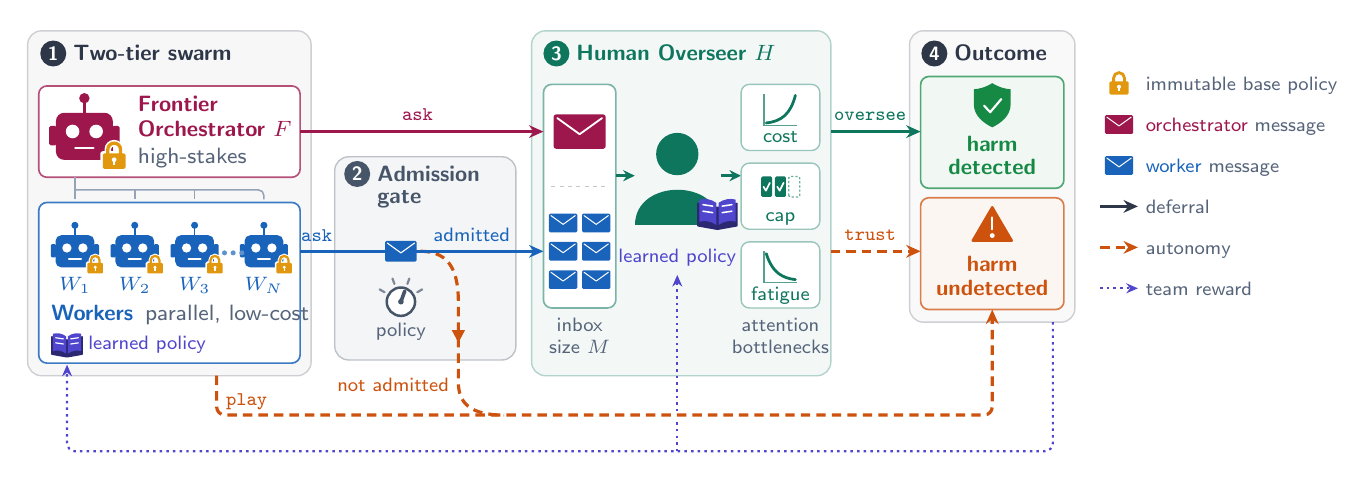
\begin{tikzpicture}[oversightfig]
\useasboundingbox (0,0.20) rectangle (16.5,5.84);

% (1) Two-tier swarm
\path[panel,fill=slate!4,draw=slate!24] (0,1.42) rectangle (3.60,5.80);
\stage{0.16}{5.42}{1}{Two-tier swarm}{slate}

% Frontier Orchestrator F (colF)
\path[card,draw=colF!75] (0.14,3.94) rectangle (3.46,5.10);
\robot{0.72}{4.46}{0.88}{colF}
\txt{1.40}{4.78}{{\fc\color{colF}Frontier}}
\txt{1.40}{4.46}{{\fc\color{colF}Orchestrator $F$}}
\txt{1.40}{4.12}{{\color{mute}high-stakes}}

\draw[disp] (0.60,3.94)--(0.60,3.66);
\draw[disp] (0.60,3.78)--(3.00,3.78)--(3.00,3.66);
\foreach \x in {1.36,2.12}{\draw[disp] (\x,3.78)--(\x,3.66);}

% Workers W_1 ... W_N (colW)
\path[card,draw=colW!85] (0.14,1.58) rectangle (3.46,3.62);
\foreach \x in {0.60,1.36,2.12,3.00}{\robot{\x}{\yW}{0.60}{colW}}
\foreach \x in {2.50,2.61,2.72}{\fill[colW!70] (\x,2.98) circle (0.032);}
\foreach \x/\l in {0.60/1,1.36/2,2.12/3,3.00/N}{\node[anchor=base,text=colW,font=\sffamily\fs] at (\x,2.50) {$W_{\l}$};}
\txt{0.30}{2.12}{{\fc\color{colW}Workers}\, {\color{mute}parallel, low-cost}}
\bookpath{0.50}{1.83}{0.36}
\node[anchor=base west,text=learnc,font=\sffamily\fs] at (0.77,1.75) {learned policy};

% (2) Admission gate
\begin{scope}[shift={(\xG,0)}]
  \path[panel,fill=gatec!6,draw=gatec!36] (0,1.62) rectangle (2.30,4.20);
  \stage{0.12}{3.89}{2}{Admission}{gatec}
  \node[anchor=base west,text=gatec,font=\sffamily\ft] at (0.54,3.61) {gate};
  \node[anchor=base,text=colW,font=\sffamily\fs] at (1.74,3.13) {admitted};
  \dial{0.84}{2.36}{0.60}{gatec}
  \node[anchor=base,text=mute,font=\sffamily\fs] at (0.84,1.92) {policy};
\end{scope}

% (3) Human Overseer H (colH)
\begin{scope}[shift={(\xH,0)}]
  \path[panel,fill=colH!5,draw=colH!32] (0,1.42) rectangle (3.80,5.80);
  \stage{0.15}{5.42}{3}{Human Overseer $H$}{colH}
  \path[card,draw=colH!55] (0.15,2.28) rectangle (1.07,5.12);
  \envelope{0.61}{\yF}{0.66}{colF}
  \draw[slate!28,line width=0.5pt,dash pattern=on 1.5pt off 1.5pt] (0.25,3.82)--(0.97,3.82);
  \foreach \y in {3.36,\yW,2.64}{\foreach \x in {0.40,0.82}{\envelope{\x}{\y}{0.36}{colW}}}
  \node[anchor=base,text=mute,font=\sffamily\fs] at (0.61,1.98) {inbox};
  \node[anchor=base,text=mute,font=\sffamily\fs] at (0.61,1.70) {size $M$};
  \person{1.85}{3.96}{1.25}{colH}
  \bookpath{2.36}{3.50}{0.46}
  \node[anchor=base,text=learnc,font=\sffamily\fs] at (1.85,2.86) {learned policy};
  \draw[hop,colH] (1.07,3.96)--(1.31,3.96);
  \draw[hop,colH] (2.40,3.96)--(2.66,3.96);
  \tile{4.28}{cost}\tile{3.28}{cap}\tile{2.28}{fatigue}
  \begin{scope}[shift={(2.95,4.60)}]
    \draw[colH!70,line width=0.5pt] (0,0.40)--(0,0)--(0.42,0);
    \draw[colH,line width=1pt,line cap=round] (0.03,0.03) .. controls (0.23,0.05) and (0.34,0.15) .. (0.40,0.38);
  \end{scope}
  \begin{scope}[shift={(2.915,3.66)}]
    \foreach \k in {0,1}{\fill[colH,rounded corners=0.5pt] (0.175*\k,0.03) rectangle (0.175*\k+0.14,0.29);
      \draw[white,line width=0.6pt,line cap=round,line join=round] (0.175*\k+0.030,0.160)--(0.175*\k+0.060,0.110)--(0.175*\k+0.110,0.210);}
    \draw[colH!60,line width=0.45pt,rounded corners=0.5pt,dash pattern=on 0.8pt off 0.7pt] (0.35,0.03) rectangle (0.49,0.29);
  \end{scope}
  \begin{scope}[shift={(2.95,2.60)}]
    \draw[colH!70,line width=0.5pt] (0,0.40)--(0,0)--(0.42,0);
    \draw[colH,line width=1pt,line cap=round] (0.03,0.37) .. controls (0.11,0.12) and (0.24,0.06) .. (0.40,0.04);
  \end{scope}
  \node[anchor=base,text=mute,font=\sffamily\fs] at (3.16,1.98) {attention};
  \node[anchor=base,text=mute,font=\sffamily\fs] at (3.16,1.70) {bottlenecks};
\end{scope}

% (4) Outcome
\begin{scope}[shift={(\xO,0)}]
  \path[panel,fill=slate!3,draw=slate!24] (0,2.10) rectangle (2.10,5.80);
  \stage{0.15}{5.42}{4}{Outcome}{slate}
  \path[card,draw=accent!75,fill=accent!6] (0.14,3.80) rectangle (1.96,5.22);
  \shield{1.05}{4.86}{0.52}{accent}
  \node[anchor=base,text=accent,font=\sffamily\fontsize{7.6}{9}\selectfont\bfseries] at (1.05,4.27) {harm};
  \node[anchor=base,text=accent,font=\sffamily\fontsize{7.6}{9}\selectfont\bfseries] at (1.05,3.97) {detected};
  \path[card,draw=warn!75,fill=warn!5] (0.14,2.26) rectangle (1.96,3.68);
  \warntri{1.05}{3.33}{0.50}{warn}
  \node[anchor=base,text=warn,font=\sffamily\fontsize{7.6}{9}\selectfont\bfseries] at (1.05,2.74) {harm};
  \node[anchor=base,text=warn,font=\sffamily\fontsize{7.6}{9}\selectfont\bfseries] at (1.05,2.44) {undetected};
\end{scope}

% Flows
\draw[flow,colF] (3.46,\yF)--(\xH+0.15,\yF);
\node[anchor=base,text=colF,font=\ttfamily\fontsize{7}{8}\selectfont] at (4.95,4.66) {ask};

\draw[fbk] (\xO+1.82,2.10)--(\xO+1.82,\yR)--(0.50,\yR)--(0.50,1.56);
\draw[fbk] (8.25,\yR)--(8.25,2.70);

\draw[white,line width=3.2pt] (8.09,\yP)--(8.41,\yP);
\draw[unrev] (2.40,1.42)--(2.40,\yP)--(\xO+1.05,\yP)--(\xO+1.05,2.26);
\node[anchor=base west,text=warn,font=\ttfamily\fontsize{7}{8}\selectfont] at (2.52,1.04) {play};

\draw[unrev,-] (\xG+1.09,\yW) .. controls (\xG+1.49,\yW) and (\xG+1.57,2.70) .. (\xG+1.57,2.24)
               -- (\xG+1.57,1.44) .. controls (\xG+1.57,1.08) and (\xG+1.71,\yP) .. (\xG+2.15,\yP);
\fill[warn] (\xG+1.57,1.84)--(\xG+1.57-0.085,2.00)--(\xG+1.57+0.085,2.00)--cycle;
\draw[flow,colW] (3.46,\yW)--(\xH+0.15,\yW);
\envelope{\xG+0.84}{\yW}{0.40}{colW}
\node[anchor=base,text=colW,font=\ttfamily\fontsize{7}{8}\selectfont] at (3.67,3.12) {ask};
\node[anchor=base east,text=warn,font=\sffamily\fs] at (\xG+1.45,1.22) {not admitted};

\draw[flow,colH] (\xH+3.80,\yF)--(\xO+0.14,\yF);
\node[anchor=base,text=colH,font=\ttfamily\fontsize{7}{8}\selectfont] at (10.70,4.66) {oversee};
\draw[unrev] (\xH+3.80,\yW)--(\xO+0.14,\yW);
\node[anchor=base,text=warn,font=\ttfamily\fontsize{7}{8}\selectfont] at (10.70,3.14) {trust};

% Legend
\begin{scope}[every node/.append style={font=\sffamily\fs,text=mute,anchor=base west}]
  \lockpath{\xL+0.24}{5.14}{0.30}          \node at (\xL+0.58,5.04) {immutable base policy};
  \envelope{\xL+0.24}{4.61}{0.36}{colF}    \node at (\xL+0.58,4.52) {{\color{colF}orchestrator} message};
  \envelope{\xL+0.24}{4.09}{0.36}{colW}    \node at (\xL+0.58,4.00) {{\color{colW}worker} message};
  \draw[flow,slate,line width=1pt] (\xL,3.57)--(\xL+0.48,3.57);   \node at (\xL+0.58,3.48) {deferral};
  \draw[unrev,line width=1pt] (\xL,3.05)--(\xL+0.48,3.05);        \node at (\xL+0.58,2.96) {autonomy};
  \draw[fbk] (\xL,2.53)--(\xL+0.48,2.53);                         \node at (\xL+0.58,2.44) {team reward};
\end{scope}
\end{tikzpicture}
\end{document}
